\documentclass[12pt,a4paper]{article}
\usepackage[UTF8]{ctex}
\usepackage{amsmath,amssymb}
\usepackage{xcolor}
\usepackage{hyperref}
\usepackage{geometry}
\usepackage{graphicx}
\geometry{margin=2.5cm}

\title{Dynamics Simulation / 动力学模拟}
\author{QuoNic}
\date{}

\begin{document}
\maketitle

\begin{center}
\textbf{Simulation / 模拟} | 难度：高级 | 预计时间：20 分钟
\end{center}

\tableofcontents
\newpage

\section{为什么需要？}

量子动力学模拟用于模拟量子系统的时间演化。

\subsection{经典局限}
\begin{itemize}
  \item 经典模拟需要指数时间，对于 $n$ 个量子比特需要 $O(2^n)$ 内存
  \item 对于大系统，经典方法效率低
  \item 精确对角化只适用于小系统
\end{itemize}

\subsection{量子优势}
\begin{itemize}
  \item 量子模拟可以在多项式时间内完成
  \item 提供指数加速
  \item 是量子化学的基础
\end{itemize}

\subsection{实际应用}
\begin{itemize}
  \item 量子化学（分子动力学模拟）
  \item 材料科学（新材料设计）
  \item 量子物理（量子多体系统）
\end{itemize}

\section{快速上手}

\begin{verbatim}
from quonic.simulation import dynamics

# 模拟量子动力学
result = dynamics(H=[[1,0],[0,-1]], t=1.0, dt=0.1)
print(f'Final state: {result.state}')
print(f'Evolution: {result.evolution}')
\end{verbatim}

\textbf{预期输出}：
\begin{verbatim}
Final state: [0.54+0.84j, 0]
Evolution: [[0.54+0.84j, 0], [0, 0.54-0.84j]]
\end{verbatim}

\section{原理详解}

\subsection{电路图}

\begin{center}
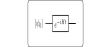
\includegraphics[width=0.6\textwidth]{../../images/dynamics_simulation_circuit.svg}
\end{center}

\subsection{数学推导}

\textbf{Step 1: 薛定谔方程}

量子系统的时间演化由薛定谔方程描述：
\begin{equation}
i\hbar \frac{d}{dt}|\psi(t)\rangle = H|\psi(t)\rangle
\end{equation}

\textbf{Step 2: 形式解}

形式解：
\begin{equation}
|\psi(t)\rangle = e^{-iHt/\hbar}|\psi(0)\rangle
\end{equation}

\textbf{Step 3: Trotter 分解}

对于大系统，使用 Trotter 分解：
\begin{equation}
e^{-iHt} \approx \prod_k e^{-iH_k \Delta t}
\end{equation}

\textbf{Step 4: 量子电路实现}

每个 $e^{-iH_k \Delta t}$ 可以用量子门实现：
\begin{equation}
e^{-iH_k \Delta t} = U_k e^{-i\lambda_k \Delta t} U_k^\dagger
\end{equation}

\textbf{Step 5: 测量}

测量量子态得到物理量：
\begin{equation}
\langle A \rangle = \langle\psi(t)|A|\psi(t)\rangle
\end{equation}

\subsection{几何解释}

量子动力学在 Bloch 球上演化量子态。哈密顿量决定旋转轴，时间决定旋转角度。

\section{代码详解}

\begin{verbatim}
from quonic.simulation import dynamics

# dynamics(H, t, dt, initial_state)
# H: 哈密顿量矩阵
# t: 总时间
# dt: 时间步长
# initial_state: 初始态

result = dynamics(
    H=[[1, 0], [0, -1]],
    t=1.0,
    dt=0.1,
    initial_state=[1, 0]
)

# result.state: 最终态
# result.evolution: 演化算子
# result.energies: 能量本征值
# result.expectation: 期望值
print(f'Final state: {result.state}')
print(f'Evolution: {result.evolution}')
\end{verbatim}

\section{进阶用法}

\subsection{场景 1：不同哈密顿量}

\begin{verbatim}
from quonic.simulation import dynamics

# 不同哈密顿量
H1 = [[1, 0], [0, -1]]  # 自旋-z
H2 = [[0, 1], [1, 0]]   # 自旋-x
H3 = [[0, -1j], [1j, 0]] # 自旋-y

for H in [H1, H2, H3]:
    result = dynamics(H, t=1.0, dt=0.1)
    print(f'Final state: {result.state}')
\end{verbatim}

\subsection{场景 2：不同时间步长}

\begin{verbatim}
from quonic.simulation import dynamics

# 不同时间步长
for dt in [0.01, 0.1, 1.0]:
    result = dynamics(H=[[1,0],[0,-1]], t=1.0, dt=dt)
    print(f'dt={dt}: Final state={result.state}')
\end{verbatim}

\section{适用场景}

\subsection{量子化学}

动力学模拟可以用于模拟分子动力学。

\subsection{材料科学}

动力学模拟可以用于设计新材料。

\subsection{量子物理}

动力学模拟可以用于模拟量子多体系统。

\section{常见问题}

\subsection{动力学模拟的精度如何？}

取决于 Trotter 分解的阶数和时间步长。

\subsection{动力学模拟需要多少量子比特？}

取决于系统的大小。

\subsection{动力学模拟和哈密顿量模拟有什么区别？}

动力学模拟关注态演化，哈密顿量模拟关注演化算子。

\section{学习路径}

\subsection{前置知识}
\begin{itemize}
  \item 哈密顿量
  \item Trotter 分解
  \item 量子测量
\end{itemize}

\subsection{继续学习}
\begin{itemize}
  \item 量子化学
  \item 材料科学
  \item 量子物理
\end{itemize}

\section{完整示例代码}

\subsection{示例 1：基本动力学模拟}

\begin{verbatim}
from quonic.simulation import dynamics

result = dynamics(H=[[1,0],[0,-1]], t=1.0, dt=0.1)
print(f'Final state: {result.state}')
\end{verbatim}

\section{下载}

\begin{itemize}
  \item [dynamics\_simulation.py](https://github.com/ChrisLee0721/QuoNic/blob/main/examples/dynamics_simulation/dynamics_simulation.py)
\end{itemize}

\end{document}
